\section{Server}
\subsection{Funktionen}
Der Server der Webapplikation muss
mehrere Aufgaben bewältigen. Ein Webserver muss \texttt{HTTP} bedienen können, um
dem Browser des Nutzers eine \HTML-Oberfläche bieten zu können. Dazu müssen
Vetretungsplan-Daten auf dem Server gepeichert, abgerufen, und bearbeitet
werden. Weiterhin muss der Server in der Lage sein, vom Nutzer hochgeladene
Dateien zu empfangen, konvertieren und zu seinen gepeicherten Daten
hinzuzufügen. Damit nur autorisierte Nutzer Daten bearbeiten können, ist eine
sichere Authenifizierung über eine Passworteingabe des Nutzers erforderlich.
Diese erforderliche Web-Sicherheit beinhält Hashwerte und die Verwendung von
\texttt{SSL}.

\subsection{Struktur}
Der Server baut auf den schon von Pyramid gegebenen Strukturen auf. In dem Webframework
sind schon viele Teile eines Servers gekapselt, sodass wir uns nicht direkt damit
außeinandersetzen mussten. Dies umfasst Authentifikation, also das Erkennen und Speichern
von Nutzern, Autorisierung, die Einschränkung aller Nutzer auf ihre Erlaubnisbereiche.
Weiterhin nimmt uns das Framework das gesamte Kommunikationsprotokolle \texttt{HTTP} ab.
Somit läuft die gesamte Kommunikation mit dem Client über Pyramid ab. Dies umfasst das Senden
von Daten via \texttt{GET}-Requests, das Empfangen von Daten durch \texttt{POST}-Requests
und die Kommunikation via \texttt{AJaX}.\\
Am Back End des Servers befinden sich die Python-Scripts. Diese haben Zugriff auf die auf dem
Server gespeicherten Daten, und steuern das Framework. Die gesamte applikationsspezifische
Programmlogik wird innerhalb dieser Scripts ausgeführt. Die Scripts bekommen Nutzerdaten von
Pyramid in Form Requests (Anfragen) vom Nutzer.
Diese verarbeiten diese je nach Art des Requests, bearbeiten gegebenenfalls die
gespeicherten Daten auf dem Server, und geben dem Framework alle Informationen für eine Antwort
an den Client. Meist bestehen diese Informationen aus einzelnen Variablen. \\Um dem Nutzer jedoch
eine Antwort zu senden, müssen diese Daten noch in ein dem Nutzer verständlichen Format wie
\texttt{HTML} gebracht werden. Diese Aufgabe wird von sogenannten Renderern erledigt. Renderer 
setzen aus einer Template (Vorlage), und den speziefischen Daten eine vollständige Antwort
zusammen. Für jeden Datensatz von den Python-Scripts, welcher an den Client gesendet werden
soll, gibt es eine bestimmte Template. So können zum Beispiel mit Leichtigkeit große,
komplexe HTML-Seiten generieren, indem man unveränderliche Bestandteile in Templates auslagert,
und nur die veränderlichen Daten der Scripts vom Renderer einsetzen zu lassen. Handelt es
sich nur um unveränderlichen Daten in einer Template, wenn es sich beispielsweise um ein reines
\texttt{CSS}-Stylesheet handelt, so ist kein Renderer von nöten. Dies wird durch sogenannte
Static Assets realisiert, welche ganze Dateien unbearbeitet dem Nutzer zur Verfügung stellen.\\
Die Applikation an sich läuft auf einem Unix-Server mit \texttt{nginx}, welches die Basis für
die \texttt{HTTP}-Kommunikation für Pyramid bildet.

\subsection{Web-Sicherheit}
Die Sicherheit des Systems steht an erster Stelle. Daher haben wir mehrere Maßnahmen ergriffen,
um unsere Applikation so sicher wie möglich zu gestalten. Die Kommunikation zwischen Server
und Client geschieht eigentlich via \texttt{HTTPS}. Dabei handelt es sich um die schon erwähnte
\texttt{HTTP}-Kommunikation, gekoppelt mit \texttt{SSL}, ein \texttt{RSA}-verschlüsseltes Protokoll,
welches ein server-spezifisches Sicherheits-Zertifikat benötigt, und globaler Standart für
Verschlüsslung im Internet ist. Dieses Protokoll ist in \texttt{nginx} implementiert, und versichert
dem Nutzer, dass kein Dritter Zugriff empfindliche Daten hat.\\\\
Die Passwörter für die verschiedenen Bereiche dürfen nur den jeweils Berechtigten bekannt sein. Dies
schließt ein Speichern der Passwörter auf dem Server in Klartext aus, da selbst wir als Programmierer
uns nicht erlauben dürfen, den Vertretungsplan zu bearbeiten. Weiterhin dürfen die Passwörter trotz
\texttt{SSL}-Verschlüsslung auch nicht in Klartext gesendet werden, da dies impliziert, dass sie im
Klartext als Wert irgenteiner Variable auf den Server-Scripten auszulesen sind. Daher werden die
Passwörter schon auf der Client-Seite von JavaScript in sogenannte Hashwerte umgewandelt.

\subsection{Bearbeitungsprozess}
Um den Vertretungsplan zu aktualisieren, werden vom verantwortlichen Lehrer ein oder mehrere
XML-Dateien auf den Server hochgeladen. Dazu ist eine Anmeldung mit dem Bearbeitungs-Passwort
erforderlich. Der Server liest daraufhin alle Dateien aus, wobei jede Datei die Informationen
für einen Tag beinhält, und fügt die Daten dem Gespeicherten hinzu oder ersetzt diese. Dabei
müssen die Daten in XML-Form in unsere Datenstruktur übertragen werden, und im JSON-Format
gespeichert werden. Dieser Prozess ist der komplexeste in der Applikation und besitzt einen
strikten Ablauf.\\
Dieser ist in folgende Schritte gegliedert:
\begin{enumerate}[itemsep=0pt]
	\item Abrufen XML-Daten
	\item Auslesen XML-Daten
	\item Konvertieren
	\item Auslesen der gespeicherten Daten
	\item Hinzufügen
	\item Speichern der Daten
	\item Antwort formulieren
\end{enumerate}
Das Verarbeiten einer hochgeladenen Datei fängt mit dem Auslesen der Datei an. Die Daten werden
in eine temporäre Datei binär überschrieben, und mit entsprechendem UTF-8 Encoding ausgelesen.
Somit sind die Daten zur weiteren Bearbeitung nur in Form eines String-Buffers in der Laufzeitumgebung
von Python vorhanden. Zeigt die hochgeladene Datei ins Leere, indem zum Beispiel der POST keine
Datei beinhält, wird ein FileNotFoundError geworfen. Konnten die Daten nicht in UTF-8
dekodiert werden, kommt ein UnicodeDecodeError. Beide Fehler werden als Fehlerstufe 
\texttt{ERROR} eingestuft (\textit{siehe Fehlerbetrachtungen}).
\\Darauf hin werden die in einem String gespeichterten XML-Daten geparst, und in ein ElementTree
-Objekt umgewandelt. Dies übernimmt das \texttt{xml.etree} Modul der Python-Standardbibliothek.
Auch hier kann ein als \texttt{ERROR} eingestufter Fehler auftreten, falls die XML-Daten z. B. auf
Grund fehlerhafter Syntax nicht geparst werden konnten.\\
Die Daten für einen Tag werden daraufhin aus dem ElementTree-Objekt über den komplexen Konvertierungsprozess
in ein Python-Dictionary umgewandelt, welches fast identisch mit dem Datenspeicherungsformat JSON ist.
Diese Konvertierung baut auf der einheitlichen Struktur der XML-Daten auf, und kann somit bei semantischen
Fehlern in den Daten einen Fehler der Stufe ERROR hervorrufen.\\
Dieser Datensatz für einen Tag soll nun dem gespeicherten Daten hinzugefügt werden. Dazu müssen erst
die alten Daten aus der gespeicherten Datei ausgelesen werden. Dabei können wieder ein FileNotFoundError
, ein syntaktischer Fehler oder ein semantischer Fehler auftreten, welche alle \texttt{CRITICAL}-Fehler sind. \\
In diesen Datensatz, der wieder als Dictionary vorhanden ist, werden nun die neuen Daten hinzugefügt, ersetzt
oder ggf. gelöscht. Dieser aktualisierte Datensatz wird daraufhin wieder in der JSON-Datei gespeichert und überschreibt
die alten Daten in der Datei.\\
Mögliche \texttt{CRITICAL}-Fehler werden nun automatisch behandelt und dem Systemadministrator weitergegeben.
Schlussendlich muss eine Antwort für den Client formuliert werden, welche ihn über das erfolgreiche bzw. misslungene
Bearbeiten der Daten informiert.


\subsection{Gegebene Datenstruktur}

Eines unserer Ziele ist, den Vertretungsplan übersichtlicher und intuitiver zu gestalten. Dazu müssen
die Informationen von Grund auf restrukturiert werden. Dazu setzten wir uns mit der Struktur der vorhandenen
Daten auseinander und entwickelten einen Konvertierungsprozess, der eine für uns sinnvolle Datenstruktur
erzeugt.\\
\paragraph{Struktur der XML-Daten}\mbox{}\\ % Neue Zeile
Die Daten können von dem Stundenplan-Verwaltungs-Programm unserer Schule in zwei verschiedenen Formen ausgegeben
werden: den Schülerplan und den Lehrerplan. Aktuell wird der Schülerplan verwendet, jedoch entschieden wir
uns für den Lehrerplan, da dieser mehr Informationen enthält und simpler strukturiert ist. Die Daten können
uns in vielen verschiedenen Formaten ausgegeben werden. Wir entschieden uns für XML, da es gut mit Python 
auszulesen ist und einfach strukturiert ist. Jeder Tag wird nach einem ganz bestimmten Schema in einer XML-Datei
repräsentiert. Im Dateikopf stehen allgemeine Informationen, von denen wir nur das Datum des betreffenden Tages
auslesen. Darauf folgen weniger relevante Daten, welche eine Auflistung aller betroffenen Lehrer und Klassen
sowie den Hofaufsichtsänderungen beinhalten. Diese ignorieren wir, da wir die enthaltenen Informationen auch
aus den restlichen Daten herleiten können, und unser Vertretungsplan primär auf Schüler ausgerichtet ist.
Der Hauptteil der XML-Datei ist eine Auflistung aller Änderungen (Aktionen) des Tages. Jede Aktion ist folgendermaßen
strukturiert:

\lstdefinelanguage{XML}{
	morestring=[s]{>}{<},
	morecomment=[s]{!--}{--},
	identifierstyle=\color[rgb]{0.0,0.0,0.6}
}

\lstset{
	language=XML,
	basicstyle=\ttfamily,
	commentstyle=\color[rgb]{0.4,0.4,0.4},
	columns=fullflexible,
	showstringspaces=false,
	tabsize=4,
}
\begin{lstlisting}
<aktion>
	<stunde></stunde>   <!-- betreffende Stunde (Zeit) -->
	<fach></fach>       <!-- normales Unterrichtsfach -->
	<lehrer></lehrer>   <!-- normaler Lehrer -->
	<klasse></klasse>   <!-- betroffene Klasse -->
	<vfach></vfach>     <!-- Vertretungsfach -->
	<vlehrer></vlehrer>	<!-- Vertretungslehrer -->
	<vraum></vraum>     <!-- Vertretungsraum -->
	<info></info>       <!-- Information als Text -->
</aktion>
\end{lstlisting}
Ein Beispiel wäre folgendes:

\begin{lstlisting}
<aktion>
	<stunde>2</stunde>
	<fach>De</fach>
	<lehrer>MI</lehrer>
	<klasse>10C</klasse>
	<vfach>Ma</vfach>
	<vlehrer>MEL</vlehrer>
	<vraum>D209</vraum>
	<info>Aufgaben im, Unterrichtsraum</info>
</aktion>
\end{lstlisting}
Diese Aktion besagt, dass in der 2. Stunde das Fach Deutsch der Klasse 10c mit Frau Mittelstädt ersetzt 
wird durch Mathematik mit Herrn Mehlhos im Raum D209. Hat das Vertretungsfach, der Vertretungslehrer oder
-raum den Wert \glqq\texttt{-{}-{}-}\grqq{} oder gar keinen Wert, dann fällt das betroffene Fach aus.

\paragraph{Klassenbezeichner}\mbox{}\\
Besonders Klassenbezeichner sind im Vertretungsplan schwer zu dechiffrieren. Daher nahmen wir die Syntax
genau auseinander und bauten von Grund auf neue Klassenbezeichnner. Folgende Zeilen sind mögliche Bezeichner
des Lehrer-Vertretungsplans:
\begin{itemize}[itemsep=0pt]
	\ttfamily
	\item[] 10C
	\item[] 06A
	\item[] 08A,08B,08C/ 08FRZ2
	\item[] 06A,06B/ 06ABET
	\item[] 10C/ 10CIF2
	\item[] 11/ ma2
	\item[] 12/ ene
\end{itemize}
Wir unterscheiden zwischen drei Typen von Bezeichnern. Der erste Typ \glqq\texttt{SIMPLE}\grqq{} ist in den ersten zwei
Beispielen zu sehen, und steht für eine normale Klasse unter Stufe 11. Dabei gibt es zwei Teile: Klassenstufe (\texttt{grade})
und Unterstufe {\texttt{subgrade}.\\
\begin{figure}[H]
	\centering
	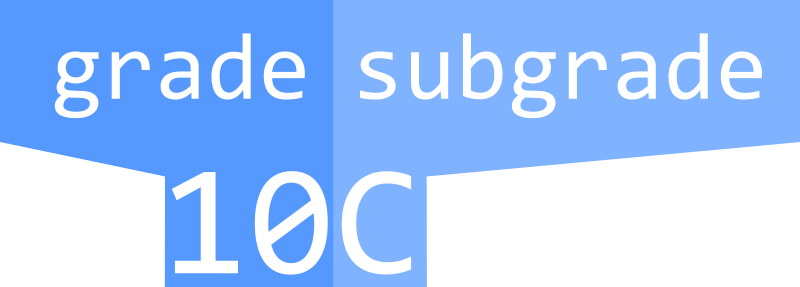
\includegraphics[height=5em]{svg/simple.png}
	\caption{Aufbau eines einfachen Bezeichners}
\end{figure}

Den zweiten Typ nennen wir \glqq\texttt{MULT}\grqq{} für \glqq multiple\grqq{}. Er bezeichnet alle Schülergruppen,
welche nicht im Klassenverband an einer Stunde teilnehmen. Dies kann entweder Klassen-intern wie das geteilte Fach
wie Informatik sein, oder Klassen-übergreifend wie Fremdprachenfächer einer Klassenstufe. Er beginnt mit einer
Aufzählung aller betroffenen Klassen (\texttt{targets}) in der Form von \texttt{SIMPLE}, und endet mit einer
allgemeinen Bezeichnung. Diese fängt immer mit der Klassenstufe (\texttt{grade}) an, kann danach gefolgt sein von
den betrefflichen Unterstufen (\texttt{subgrades}), hat danach immer das entsprechende Fach (\texttt{subject}) und
endet ggf. mit einer Gruppennummer (\texttt{subclass}). \\
\begin{figure}[H]
	\centering
	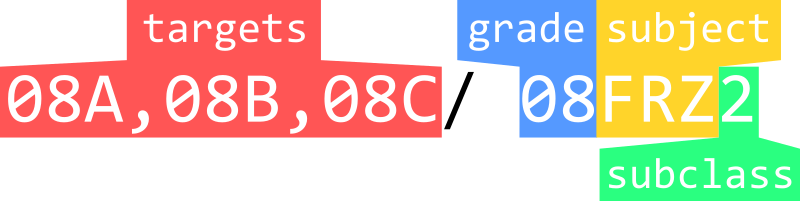
\includegraphics[height=5em]{svg/mult1.png}
	\caption{Aufbau eines Mehrfach-Bezeichners}
\end{figure}
\vspace{2em}
\begin{figure}[H]
	\centering
	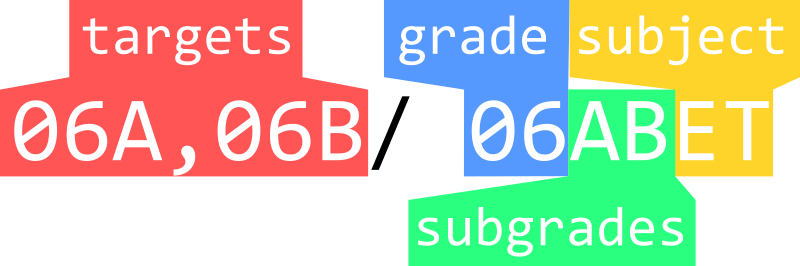
\includegraphics[height=5em]{svg/mult2.png}
	\caption{Aufbau eines Kurs-Bezeichners}
\end{figure}

Der dritte Typ \glqq\texttt{COURSE}\grqq{} beschreibt alle Kurse. Er besteht immer Klassenstufe 11 oder 12, einem
Kurs und einem Fach und einer optionalen Kursnummer am Ende.\\
Diese Unterteilung betrachtet jedoch keine AG's, WoU's, oder E- und Z-Kurse. Daher sind die Fächer an sich, wie sie
als Element in jedem Bezeichner auftreten können, nochmals unterteilt. Ein Fach besteht dabei immer aus dem Namen
als Abkürzung und einem optionalen Prefix und Suffix. So sind AG und WoU als Prefix und E- und Z-Kurse als Suffix
implementiert. Dies ist allerdings noch erweiterbar.

\newpage
\subsection{Speicherformat}
Um die ausgelesenen Einzelinformationen eines Datensatzes dauerhaft speichern zu können, speichern wir sie in unserer
eigenen Datenstruktur als JSON-Datei. Dabei gibt es eine globale Datei namens \texttt{schedule.json}, welche alle
Informationen aller Tage beinhält. Ihr einziges Element ist eine Liste aller Tage. Jeder Tag ist folgendermaßen
gegliedert:

\lstdefinelanguage{JSON}{
	morestring=[s]{"}{"},
	morecomment=[s]{/*}{*/},
	alsoletter=0123456789,
}

\lstset{
	language=JSON,
	basicstyle=\ttfamily,
	stringstyle=\color[rgb]{0.0,0.0,0.6},
	commentstyle=\color[rgb]{0.4,0.4,0.4},
	columns=fullflexible,
	showstringspaces=false,
	tabsize=4,
}
\lstset{literate=% Shamelessly stolen from textwelt.de to escape umlauts in listings
  {Ö}{{\"O}}1
  {Ä}{{\"A}}1
  {Ü}{{\"U}}1
  {ß}{{\ss}}2
  {ü}{{\"u}}1
  {ä}{{\"a}}1
  {ö}{{\"o}}1
}
\begin{lstlisting}
{
	"date": {
		"day": 19,
		"month": 10,
		"year": 2015
	},
	"events": [...],
	"filename": "VplanLe19102015.xml"
}
\end{lstlisting}
Es ist ein Datum für den betreffenden Tags angegeben, der Dateiname für Nutzerinformation, und ein Array welches
alle einzelnen Ereignisse \jsonstr{change} enthält. Jedes Event ist folgendermaßen aufgebaut.
\begin{lstlisting}
{
	"change": "SUBJECT",
	"info": "Aufgaben im Unterrichtsraum",
	"new": {...},
	"old": {...},
	"room": "D309",
	"selector": {...},
	"targets": "6 6b Es Es Drm Drm",
	"time": "1"
}
\end{lstlisting}
Jedes Ereignis besitzt eine Information \jsonstr{change} darüber, welcher Änderungen vorgenommen wurden. Dabei 
gibt es vier verschiedene Änderungstypen mit jeweils speziefischen Kriterien.
\begin{figure}[H]
	\centering
	\begin{tabular}{r@{\quad}l@{\vspace{2mm}}}
		Typ & Kriterien \\
		\hline
		\jsonstr{SUBJECT} & Unterrichtsfach wurde geändert \\
		\jsonstr{TEACHER} & Unterrichtslehrer wurde gewechselt \\
		\jsonstr{ROOM}    & Raumwechsel \\
		\jsonstr{CANCELLED} & Stunde fällt aus \\
	\end{tabular}
\end{figure}
\newpage

Weiterhin beinhält ein Ereignis Information über die zwei betreffenden Stunden: die ursprüngliche Stunde \jsonstr{old}
und die Vertretungsstunde \jsonstr{new}. Jede dieser Stunden hat die selbe Struktur:
\begin{lstlisting}
{
	"subject": {
		"prefix": null,
		"subject": "De",
		"suffix": null
	},
	"teacher": {
		"full": "Frau Mittelstädt",
		"short": "Mi"
}
\end{lstlisting}
Eine Stunde enthält ein Fach \jsonstr{subject} und einen Fachlehrer \jsonstr{teacher}. Das Fach besteht wie schon
oben beschrieben aus dem Fachnamen als Abkürzung, sowie einem optionalem Präfix und Suffix. Der Lehrer ist sowohl
als Abkürzung \jsonstr{short} als auch als vollständiger Name \jsonstr{full} dargestellt.\\
Die betreffende Klasse bzw. Schülergruppe ist im Bezeichner \jsonstr{selector} gespeichert. Es gibt drei Typen von
Selektoren, \jsonstr{SIMPLE}, \jsonstr{MULT} und \jsonstr{COURSE}, welche wir schon klassifiziert und mit jeweiligen
Attributen versehen haben. Daher ist jeder Selektor aus den selben vier definierenden Attributen aufgebaut, sowie
einer Information über den betreffenden Typ. Nutzt ein Typ ein Attribut nicht, so wird diesem
der Wert \texttt{\color[rgb]{0.0,0.0,0.6}{null}} zugewiesen. Hier ein Beispiel für einen Selektor vom Typ \jsonstr{SIMPLE}:
\begin{lstlisting}
{
	"grade": 6,
	"subclass": null,
	"subgrades": "b",
	"subject": null,
	"type": "SIMPLE"
}
\end{lstlisting}
Ein Ereignis beinhält weiterhin ein \jsonstr{targets}-Attribut, welches in einem String durch Leerzeichen separiert alle
betreffenden Klassen und Lehrer für die Filter-Funktion beinhält. Natürlich wird auch die Zeit der Stunde gespeichert.
Falls es sich um Mehrfach-Stunden handelt, so werden beide Ereignisse zu einem zusammengezogen, und die Zeitangabe wird
durch ein mit \texttt{-} getrenntes Zeitintervall getrennt. Ist eine Textinformation vorhanden, so wird diese ebenfalls
in \jsonstr{info} abgelegt.

\subsection{Fehlerbehandlung und Logging}
Der Verarbeitungsprozess besteht aus mehreren Schritten, die jeweils einzelne Fehlerbetrachtungen
und ausführliche Logs haben. Jeder mögliche Fehler wird abgefangen, geloggt und ggf. automatisch 
behandelt. Dabei werden die Fehler in drei Log-Level unterteilt: \texttt{WARNING}, das niedrigste Level,
welches einen Fehler beschreibt, der unerwünscht ist, jedoch die Gesamtheit der Daten des Tages
nicht gravierend beeinträchtigt, \texttt{ERROR}, ein Fehler, der das Abbrechen der Bearbeitung und somit
den Fehlen des jew. Tages zur Folge hat, und \texttt{CRITICAL}, die höhste Fehlerstufe, welche nur komplett
unerwartete Fehler die die gesamte Funktionalität der Applikation beeinträchtigen umfasst.
Bei \texttt{CRITICAL}-Fehlern wird zudem automatischematisch eine Email an die System-Administratoren geschickt,
und, wenn möglich, eine automatische Wiederherstellung des Systems eingeleitet.